\section{Virtual Memory}
We expose a virtual memory space to applications so that they can
assume that they own the whole space, then the OS handles the mapping of virtual
to physical memory space. Every program will have its own virtual address space
that is protected from other programs. Frequently-used portions of virtual address
space copied to DRAM.

\textbf{Page Table:} A data structure which contains virtual to physical address
mappings. If we haven't used a page in a while we can map it to disk memory instead
of DRAM. Page tables are mapping in a coarser granularity i.e 4Kb

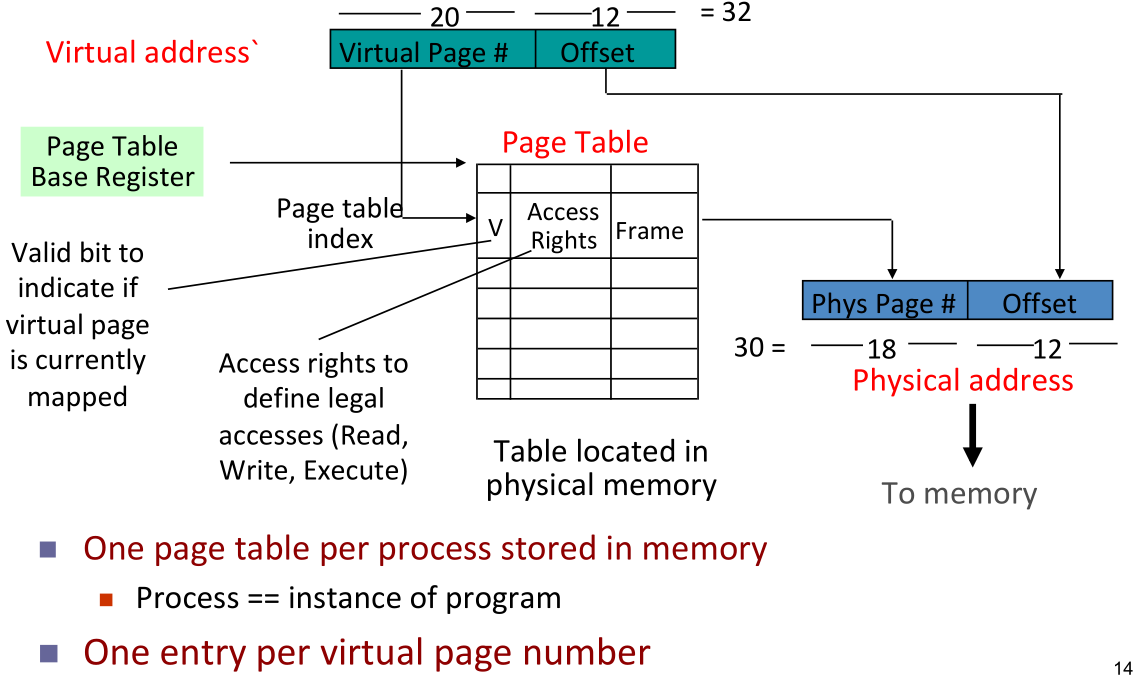
\includegraphics[width=\linewidth]{png/pagetable.png}

\textbf{TLB} is a hardware cache just for translation entries for page tables,
locality in accesses $\rightarrow$ locality in translations. Each TLB entry stores
a page table entry (PTE), the data that is stored is
\textbf{physical page numbers, permission bits (RXW), other PTE info (dirty bit, etc.)}

\textbf{TLB Organization}

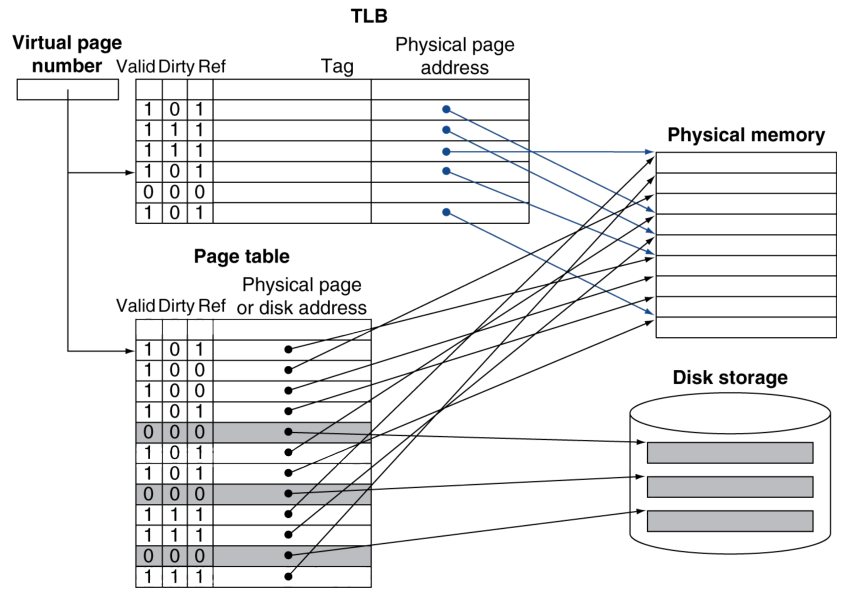
\includegraphics[width=\linewidth]{png/tlb.png}

\textbf{Virtually Indexed, Physically Tagged Cache}

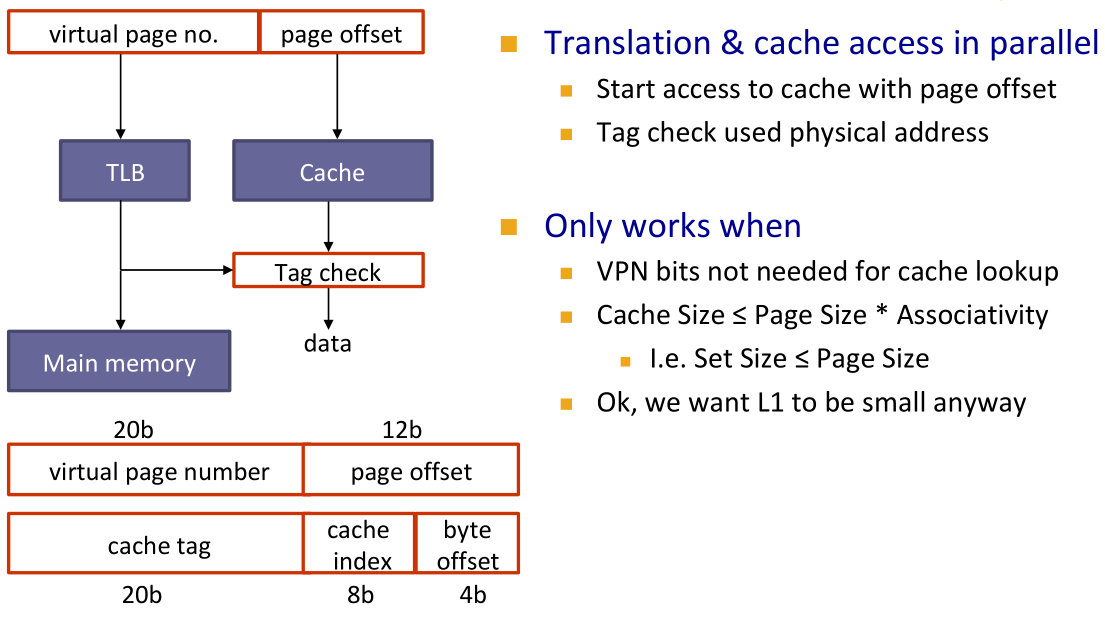
\includegraphics[width=\linewidth]{png/tlblook.png}
